\section{Results}\label{sec:results}

All risks in RQ1 and RQ2 are with respect to construction labels on development data (Section~\ref{sec:problem}); coverage and risk use the 258 labelled pairs as denominator, and confidence intervals are 95\% project-cluster bootstrap intervals. Numbers are for cross-validation seed~0 on the Linux-branch code unless stated otherwise; Section~\ref{sec:res-robust} reports variability across seeds and the effect of the profile fix.

\subsection{RQ1: Coverage and Risk of Decision Rules}
The upper block of Table~\ref{tab:ablation} and the point markers in Fig.~\ref{fig:riskcov} show the rule baselines. Plain differential testing (B1) issues \NDO{} on 183 of 258 labelled pairs (coverage 0.709), of which 31 have $Y{=}1$: an observed false-assurance risk of 0.169 [0.086, 0.354]. In other words, roughly one in six ``no difference'' outcomes concealed a labelled behavioural change, even though every one of them would have been reported as a clean comparison. Requiring deterministic witnesses (B2) changes nothing on these data. Counting the unlabelled pairs that received \NDO{} as false assurances gives worst-case risks of 0.333 (B1), 0.324 (B3), 0.225 (B4) and 0.227 (B5).

The V7-B sufficiency gate (B3) abstains much more: it issues 61 \NDO{} verdicts (coverage 0.236), of which 13 are wrong, a risk of 0.213 [0.090, 0.457]. Abstaining on three quarters of the B1 verdicts did \emph{not} lower the risk among the verdicts that remained. The simpler coverage gates do better on this sample: requiring full activation and the branch-coverage floor (B4) issues 141 verdicts at risk 0.121 [0.044, 0.343], and coverage-gated B1 (B5) 144 at 0.125 [0.052, 0.343]. All intervals overlap substantially, so the ordering is suggestive only; the clearest finding is negative. The V7-B gate's additional blocking conditions removed many verdicts without removing a disproportionate share of the wrong ones, which is exactly the failure mode that matched-coverage evaluation is designed to expose.

\begin{table*}[!t]
\caption{Development-set comparison of SBG V8 decision rules, calibrated models and ablations (seed 0, out-of-fold).}
\label{tab:ablation}
\centering
\footnotesize
\begin{tabular}{|l|c|c|c|c|c|c|}
\hline
Method & Coverage & \#NDO & FA risk [95\% CI] & Brier & Log loss & Cal.\ slope \\
\hline
\multicolumn{7}{l}{\emph{Rule baselines (all 258 labelled pairs; policy-independent)}} \\
Plain differential testing (B1) & 0.709 & 183 & 0.169 [0.086, 0.354] & -- & -- & -- \\
B1 + repetition (B2) & 0.709 & 183 & 0.169 [0.086, 0.354] & -- & -- & -- \\
V7-B sufficiency gate (B3) & 0.236 & 61 & 0.213 [0.090, 0.457] & -- & -- & -- \\
Coverage-only gate (B4) & 0.547 & 141 & 0.121 [0.044, 0.343] & -- & -- & -- \\
Coverage-gated B1 (B5) & 0.558 & 144 & 0.125 [0.052, 0.343] & -- & -- & -- \\
Random abstention (B6)$^\dagger$ & 0.236 & 61 & 0.169 & -- & -- & -- \\
\hline
\multicolumn{7}{l}{\emph{Soft blockers (v8.0): 85 eligible labelled pairs}} \\
Coverage-only calibration (B7) & 0.236$^\ast$ & 61 & 0.230 [0.108, 0.465] & 0.225 & 0.649 & -1.83 \\
\quad + multiplicity & 0.236$^\ast$ & 61 & 0.292 [0.151, 0.471] & 0.219 & 0.637 & -0.03 \\
Multiplicity only & 0.236$^\ast$ & 61 & 0.295 [0.151, 0.473] & 0.212 & 0.620 & 0.21 \\
CEC without ERS (B9) & 0.236$^\ast$ & 61 & 0.292 [0.151, 0.468] & 0.221 & 0.645 & -0.02 \\
CEC with ERS (B8) & 0.236$^\ast$ & 61 & 0.213 [0.124, 0.392] & 0.207 & 0.615 & 0.30 \\
\hline
\multicolumn{7}{l}{\emph{Strict blockers (v8.0s $\equiv$ v8.1): 61 eligible labelled pairs}} \\
Coverage-only calibration (B7) & 0.236$^\ast$ & 61 & 0.213 [0.129, 0.473] & 0.205 & 0.615 & -4.42 \\
\quad + multiplicity & 0.236$^\ast$ & 61 & 0.213 [0.130, 0.446] & 0.188 & 0.583 & -0.11 \\
Multiplicity only & 0.236$^\ast$ & 61 & 0.213 [0.129, 0.446] & 0.189 & 0.587 & -0.17 \\
CEC without ERS (B9) & 0.236$^\ast$ & 61 & 0.213 [0.130, 0.446] & 0.188 & 0.583 & -0.11 \\
CEC with ERS (B8) & 0.236$^\ast$ & 61 & 0.213 [0.125, 0.443] & 0.182 & 0.578 & 0.05 \\
\hline
\end{tabular}
\\[2pt]
\parbox{\textwidth}{\scriptsize DEVELOPMENT DATA, EXPLORATORY, NOT INDEPENDENT VALIDATION. Split: development only (312 pairs, 258 with construction labels, 54 unlabelled and excluded, 101 labelled projects, 114 overall; quixbugs = 43.8\% of labelled pairs). Coverage and FA risk are over the 258 labelled pairs; 95\% CIs are percentile project-cluster bootstrap intervals (10{,}000 resamples). $^\ast$Model rows are rank-matched to the V7-B gate coverage $c^*=61/258$ (transductive diagnostic, not a deployable threshold); with nested-CV thresholds at $\alpha\in\{0.10,0.15\}$ the models issue 0 NDO (multiplicity-only: 1). Under strict blockers every model issues exactly V7-B's 61 NDO pairs, so risks are identical by construction; their CIs use only the ${\approx}50\%$ of resamples in which $c^*$ is attainable and are therefore not reliable. Brier, log loss and slope are on eligible pairs only (out-of-fold base-rate Brier 0.230 soft, 0.205 strict). $^\dagger$Expected risk of random abstention among B1-issuable pairs. Per-method runtime was not recorded; the whole 13-system evaluation took 109--117\,s per seed (Linux run). Linux-branch code, before the mac-branch ERS profile fix.}
\end{table*}


\begin{figure}[!t]
\centering
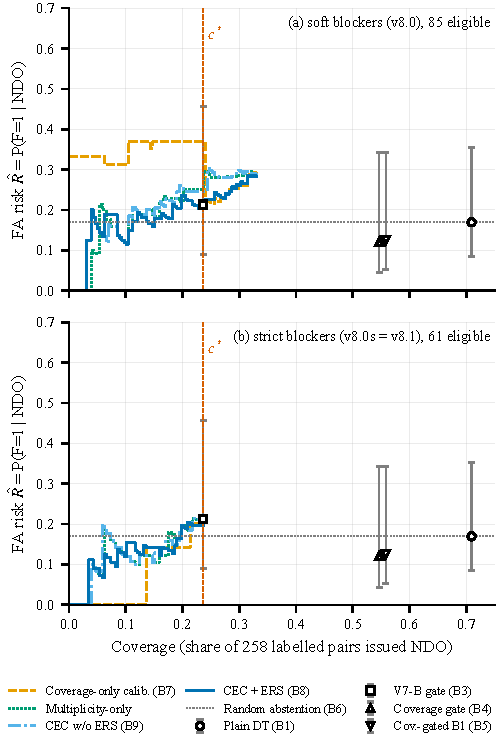
\includegraphics[width=\columnwidth]{figures/fig_risk_coverage.pdf}
\caption{Risk--coverage curves for the calibrated models (out-of-fold, seed~0) under (a) soft and (b) strict blocker policies, with rule baselines as points (95\% project-cluster bootstrap intervals). The vertical line marks the matched coverage $c^\ast=61/258$ of the V7-B gate. The calibrated curves end at the share of eligible pairs (85 soft, 61 strict).}
\label{fig:riskcov}
\end{figure}

\subsection{RQ2: Does the Evidence Profile Reduce False-Assurance Risk?}
\paragraph*{Matched-coverage risk} At $c^\ast$, under the soft policy, full \cec{} with \ers{} features (B8) has observed risk 0.213 [0.124, 0.392], against 0.230 for coverage-only calibration (B7), 0.292 for \cec{} without \ers{} (B9) and 0.295 for multiplicity alone. The pre-registered primary contrast, B7 minus B8, is $+1.6$ percentage points in favour of \cec{}, with 95\% interval $[-6.6, +16.3]$. Hypothesis H2, which required a reduction of at least 5 points with a positive lower bound, is not supported. \cec{} with \ers{} ties the V7-B gate at this coverage (difference $0.0$, $[-6.2, +16.2]$) and its observed risk is 4.4 points above the expected risk of random abstention among B1-issuable pairs (0.169); this contrast is not significant. Fig.~\ref{fig:forest} shows these contrasts. In the pre-registered three-test family the Holm-adjusted $p$ is at least 0.46 in every soft-policy seed. None of the eight recomputed contrasts reaches unadjusted one-sided significance at 0.05 in either policy, and after Holm adjustment the smallest $p$ is 0.68 (soft) and 1.0 (strict).

Under the strict policy every calibrated model is confined to V7-B's own 61 \NDO{} pairs, so at $c^\ast$ all of them issue exactly that set and have identical risk 0.213. The strict-policy matched-risk contrasts are therefore zero by construction, and their bootstrap intervals are not meaningful: in roughly half of the resamples $c^\ast$ exceeds the eligible share and the resample is dropped, which produces intervals that can exclude zero around a point estimate of exactly zero. We report only the point estimate for these contrasts.

\paragraph*{Probabilistic accuracy} On the 85 soft-eligible pairs, full \cec{} has the lowest out-of-fold Brier score (0.207) and log loss (0.615) of the calibrated models, against an out-of-fold base-rate Brier score of 0.230. The improvement of the profile over coverage-only calibration (H1a, B7 vs.\ B9) is $+0.003$ in log loss $[-0.083, +0.058]$. The improvement attributable to \ers{} features (H3, B9 vs.\ B8) is $+0.030$ $[-0.014, +0.085]$. Neither interval excludes zero, so neither hypothesis is supported. On the mac-hardening branch, a placebo test that permutes the \ers{} features 100 times found the observed log-loss gain above the 95th percentile of the permutation distribution in five of six policy--seed runs (permutation $p$ between 0.01 and 0.03; $p=0.21$ in the sixth). We regard this as weak, unadjusted evidence that the \ers{} responses carry some signal beyond noise, insufficient to establish a predictive advantage given that the paired bootstrap intervals include zero in five of the six runs.

\paragraph*{Calibration} Calibration slopes are unstable and uninformative at this sample size (Fig.~\ref{fig:calibration}). For full \cec{} the slope is 0.30 with a cluster-bootstrap interval of $[-0.46, 1.13]$; for coverage-only calibration it is $-1.83$, meaning that its out-of-fold risk ordering is \emph{inverted} relative to the observed miss rates. A slope below 1 indicates over-dispersed predictions; a negative slope indicates that the model ranks pairs in the wrong order. The quantile reliability bins contain about 17 pairs each and have wide Wilson intervals.

\paragraph*{Deployable thresholds} When thresholds are chosen as specified---on inner folds, with a cluster-bootstrap upper bound on risk below $\alpha$---no calibrated model issues any \NDO{} verdict at $\alpha\in\{0.10, 0.15\}$, except multiplicity-only, which issues one. On this corpus the evidence is too weak, and the sample too small, for the conservative rule to certify any verdict. On the mac-hardening branch a frozen-threshold study fitted thresholds on training projects and applied them unchanged to held-out projects: the conservative rule again issued nothing, and the optimistic rule that uses the point estimate of risk produced held-out risks between 0.24 and 0.50 against targets of 0.10--0.20. No calibrated model achieved risk control.

\begin{figure}[!t]
\centering
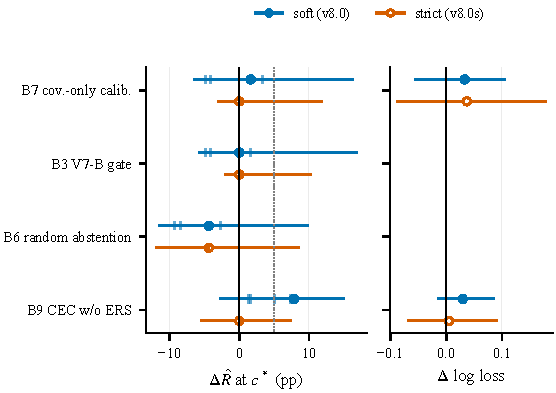
\includegraphics[width=\columnwidth]{figures/fig_ablation_forest.pdf}
\caption{Paired contrasts with full \cec{} (B8) at matched coverage $c^\ast$ (left, percentage points) and in out-of-fold log loss (right). Positive values favour B8. Dots: seed~0 with 95\% project-cluster bootstrap intervals; ticks: seeds 1--4. The dotted line marks the 5-point margin of hypothesis H2. Strict-policy matched-risk intervals use only resamples in which $c^\ast$ is attainable and are shown for completeness only.}
\label{fig:forest}
\end{figure}

\begin{figure}[!t]
\centering
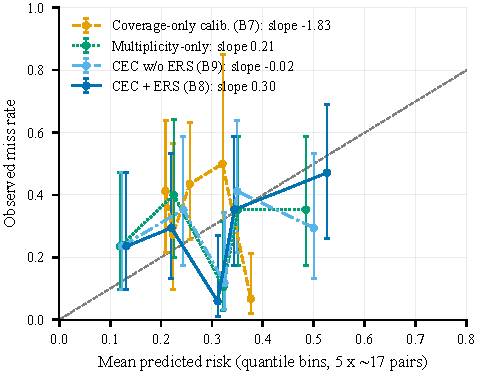
\includegraphics[width=\columnwidth]{figures/fig_calibration.pdf}
\caption{Reliability diagram for the calibrated models (soft policy, seed~0, out-of-fold, five quantile bins of about 17 eligible pairs, Wilson 95\% intervals). Legend values are logistic calibration slopes.}
\label{fig:calibration}
\end{figure}

\subsection{Robustness, Seeds and Power}\label{sec:res-robust}
\paragraph*{Seeds} Across five cross-validation seeds the primary soft-policy difference B7 minus B8 at $c^\ast$ is $+1.6$, $+1.6$, $+3.3$, $-4.1$ and $-4.9$ points (mean $-0.5$); its sign is not stable. The \ers{} log-loss gain ranges from 0.005 to 0.030 and its interval includes zero in all five soft-policy seeds and in four of five strict-policy seeds (the fifth, seed 2, is affected by the strict-policy bootstrap degeneracy). Full \cec{} log loss is $0.600\pm0.023$ and its calibration slope $0.47\pm0.20$.

\paragraph*{Profile fix} The Linux-branch numbers were produced by the pre-fix profile; they coincide with the corresponding mac-branch pre-fix runs to $10^{-9}$. Re-running with the fixed profile (mac-hardening branch) left seeds 0 and 1 of the soft policy unchanged, moved seed~2's log loss from 0.624 to 0.620 and its primary difference from $+3.3$ to $0.0$ points, and changed \ers{} log-loss gains by at most 0.008. No conclusion changes.

\paragraph*{Power} The 61 \NDO{} verdicts of the reference set fall into 34 clusters with an intra-cluster correlation of 0.61, a design effect of 1.48 and an effective sample size of about 41. The minimum paired difference in false-assurance risk detectable with 80\% power is 13.5, 16.5 and 21 percentage points at discordant shares of 0.10, 0.15 and 0.25 (Fig.~\ref{fig:power}). Detecting the pre-registered 5-point improvement would require about 460, 690 or 1{,}160 issued \NDO{} verdicts respectively---roughly 8 to 19 times the present set. The non-significant results above therefore say little about whether an effect of practically relevant size exists.

\begin{figure}[!t]
\centering
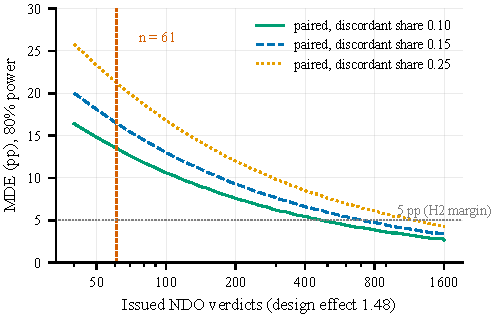
\includegraphics[width=\columnwidth]{figures/fig_power_mde.pdf}
\caption{Minimum detectable paired difference in false-assurance risk (80\% power, two-sided $\alpha=0.05$, design effect 1.48) as a function of the number of issued \NDO{} verdicts. The vertical line marks the present $n=61$; the dotted line marks the 5-point margin of H2.}
\label{fig:power}
\end{figure}

\subsection{RQ3: Conformance to the Evidence Response Signature}
Table~\ref{tab:ers} reports the property matrix on all 312 development records for six predictors. Three findings stand out.

\paragraph*{The matrix detected a profile defect} The all-feature probe, an unfitted model that reads every profile feature with its pre-declared sign, failed irrelevant-evidence invariance (P2) on 109 of 227 applicable records: appending two inputs that reach only unchanged lines \emph{lowered} its estimated risk by up to 0.32. The cause was the profile, not the probe: quantity and diversity features counted inputs that reach no changed unit. After the profile was restricted to relevant evidence (Section~\ref{sec:approach}), the probe passed P2 on all 227 records with $\Delta$ exactly zero, and no other cell of the matrix changed. The fitted model had passed P2 throughout, but only because it happens to retain essentially one feature (\code{mu\_min}) that irrelevant inputs cannot move; the defect would have surfaced in any model that used the quantity features. This is the intended use of \ers{} as a conformance test: it caught a defect that aggregate metrics did not, because the defect does not change any prediction of the fitted model on unperturbed data.

\paragraph*{The matrix separates decision procedures} Replaying the recorded V7-B verdict fails divergence responsiveness (P6) on 71 records (its 157 passes rest entirely on stored \INS{} verdicts, i.e.\ abstention credit) and integrity sensitivity (P8) on 155: a stored verdict cannot react to new evidence. Re-applying the V7-B gate to the perturbed record repairs P6 but still fails P8 on 84 records, every one a witnessed divergence that V7-B keeps as \DIV{} even when the evidence is marked as tampered. The \sbg{} trust gate forces \INS{} on any integrity failure and passes P8 on all 312 records. This rule was itself added after a first run of the matrix showed the same 84 failures for an earlier version of the \sbg{} decision procedure.

\paragraph*{Responses are real but concentrated} For the fitted model, no monotone pass rests on abstention credit; its risk rose beyond tolerance in 9 of 16 P1 trials, 68 of 93 P1b trials and 100 of 176 P5 trials, and was unchanged for P4, P7 and P9. The fitted model therefore responds to the loss of relevant evidence and to reduced reproducibility, but on this corpus it is indifferent to channel loss, provenance and environment, because those features were constant in the training data. P1 is applicable to only 16 records, because few records have a single input that is the sole reacher of a changed unit.

% Source: results/v8/linux/perturb/posthoc_matrix.{json,md} (Linux branch, pre-fix profile) and, for the probe after the profile fix,
% research/v8-mac-hardening@b9b8a86c:results/v8_mac_perturb_profilefix2/posthoc_matrix.md. Driver: experiments/v8/run_perturbation_validation.py.
\begin{table*}[!t]
\caption{\ers{} property matrix on the 312 development records (post-hoc perturbations of recorded evidence). Each cell gives the number of passes among the applicable trials; N/A trials are excluded. ``Resp.'' is the number of applicable trials in which the fitted model's risk moved by more than the tolerance. Failures are in bold.}
\label{tab:ers}
\centering
\footnotesize
\setlength{\tabcolsep}{4pt}
\begin{tabular}{|l|l|c|c|c|c|c|c|c|c|}
\hline
 & & & \multicolumn{2}{c|}{Fitted profile model} & \multicolumn{2}{c|}{All-feature probe} & & \multicolumn{2}{c|}{V7-B gate} \\
Id & Property & Applicable & Pass & Resp. & Pre-fix & Post-fix & Activation stub & Recorded & Recomputed \\
\hline
P1 & Relevant-evidence sensitivity & 16 & 16 & 9 & 16 & 16 & 16 & 16 & 16 \\
P1b & Relevant-evidence sensitivity & 93 & 93 & 68 & 93 & 93 & 93 & 93 & 93 \\
P2 & Irrelevant-evidence invariance & 227 & 227 & 0 & \textbf{118} & 227 & 227 & 227 & 227 \\
P3 & Duplicate-evidence invariance & 262 & 262 & 0 & 262 & 262 & 262 & 262 & 262 \\
P4 & Observation-loss sensitivity & 178 & 178 & 0 & 178 & 178 & 178 & 178 & 178 \\
P5 & Reproducibility sensitivity & 176 & 176 & 100 & 176 & 176 & 176 & 176 & 176 \\
P6 & Divergence responsiveness & 228 & 228 & 0 & 228 & 228 & 228 & \textbf{157} & 228 \\
P7 & Provenance sensitivity & 178 & 178 & 0 & 178 & 178 & 178 & 178 & 178 \\
P8 & Integrity sensitivity & 312 & 312 & 0 & 312 & 312 & 312 & \textbf{157} & \textbf{228} \\
P9 & Environment sensitivity & 228 & 228 & 0 & 228 & 228 & 228 & 228 & 228 \\
\hline
\end{tabular}
\\[3pt]
\parbox{\textwidth}{\scriptsize Fitted model: $L_2$ logistic regression on the full profile, with a diagnostic threshold at the 30th percentile of in-sample eligible risk so that \NDO{} verdicts exist to be withdrawn; it is not a deployment threshold, and no pass in this column rests on abstention credit. All-feature probe: an \emph{unfitted} model that reads every profile feature with its pre-declared sign; it exists because the fitted model retains essentially one feature (\code{mu\_min}), which makes invariance checks on the other features vacuous for it. Post-fix: after restricting features to relevant evidence and collapsing unflagged copies (mac-hardening branch, commit \code{b9b8a86c}); only the P2 row changed for any predictor. Activation stub: risk $=1-a(\Ev)$. V7-B ``recorded'' replays the stored verdict and therefore ignores the perturbed evidence by construction; ``recomputed'' re-applies the V7-B gate to the perturbed record.}
\end{table*}


\subsection{RQ4: Evidence Integrity Under Attack}
Table~\ref{tab:security} and Fig.~\ref{fig:security} summarise the adversarial evaluation.

\paragraph*{Original attack suite} The original suite contains 15 attacks against a pair whose honest verdict is \DIV{}. Before hardening, on macOS, 3 were blocked, 9 detected, 1 had no effect and 2 succeeded: hiding a standard-output divergence by patching the harness's capture object (A08), and editing an unverified evidence field and re-binding the sidecar after recomputing the hash chain (P04). The independent capture and the anchor were introduced in response, and both attacks are now detected and force \INS{}. Four further attacks were added. One of them, re-chaining and re-anchoring with the anchor key (P08), succeeds by design: it is outside the threat model.

\paragraph*{Re-run at the final commit} We re-executed the suite and six evaluation-awareness probes at the final commit on macOS. Of 25 attacks and probes, 3 were blocked, 15 detected, 5 had no effect and 2 succeeded. Of the 15 detections, 10 force \INS{} through the trust gate and 5 are \emph{detection only}: patching the harness canonicaliser (A01), forging a result through the harness (A02), sensing the harness from the main module (A07), substituting another program's genuine evidence (P06) and sensing the module specification (SENSE04c) are caught only by the optional shadow or source-binding checks, and the effective verdict remains a false \NDO{}. The two successes are the out-of-scope key-holder forgery (P08) and a new file-path sensing variant, SENSE04b, that reads the real path of the variant from compiled code objects and behaves differently under analysis; it produces a false \NDO{} with no check firing. The fix for the original file-path sensing attack (SENSE04), which sanitises \code{\_\_file\_\_} and \code{sys.argv}, is therefore partial; anonymised temporary file names would close this channel and are not yet implemented. One detected attack (A17, forging a tee record with a guessed nonce) turns a true \DIV{} into \INS{}: a denial of a true divergence rather than a false assurance.

\paragraph*{Linux probes} A Linux suite, run before the SENSE04 fix, contains 51 tamper probes and 74 isolation probes (named ``container'' in the result file; no container runtime is invoked). All 51 tamper probes were detected; they comprise 24 distinct operations, and the five substitution probes were detected only through source binding. Of the 74 container probes, 8 left the true verdict intact, 1 (SENSE04) produced a false \NDO{}, and 65 ended in \INS{} with no recorded cause, after about 0.2\,s each instead of the 0.7--3.1\,s of runs that reached a decision. These 65 include probes whose code should have produced \DIV{}. They are fail-safe---none produced a false \NDO{}---but they show that the runs did not reach a decision, not that isolation blocked the attacks, and we do not count them as evidence of isolation. The Linux results file records no host, sandbox configuration or timestamp, and no Linux re-run after the remediations exists.

\paragraph*{Security position} Against adversaries A1--A3, the verified position is: fail-safe evidence integrity against post-hoc writers that do not hold the anchor key; prevention of result-channel attacks and of the tested standard-output tampering; detection, but not prevention, of in-process harness forgery and of evidence substitution; and at least one open evaluation-awareness channel. We make no claim about isolation on Linux beyond network unsharing and a read-only root, and no claim of security against arbitrary adversarial programs.

% Sources: research/v8-mac-hardening results/v8_mac_security/attack_suite_{before,after}.json; audit/security_rerun_darwin.json;
% results/v8/linux/expanded_security_suite_results.json; classification in audit/security_outcomes.json (scripts/build_security_outcomes.py).
\begin{table}[!t]
\caption{Adversarial evaluation outcomes. Controls excluded. ``Det.\ only'' counts detections by optional reviewer checks that leave a false \NDO{} as the effective verdict.}
\label{tab:security}
\centering
\scriptsize
\setlength{\tabcolsep}{2.2pt}
\begin{tabular}{|L{2.15cm}|c|c|c|c|c|c|}
\hline
Suite (platform) & $n$ & Blocked & \makecell{Detected\\(det.\ only)} & \makecell{No\\effect} & Succ. & \makecell{\INS{},\\cause\\unrec.} \\
\hline
Original, before hardening (macOS) & 15 & 3 & 9 (4) & 1 & 2 & -- \\
Original + hardening attacks, after (macOS) & 19 & 3 & 14 (4) & 1 & 1 & -- \\
Re-run at final commit incl.\ sensing probes (macOS) & 25 & 3 & 15 (5) & 5 & 2 & -- \\
Tamper probes (Linux) & 51 & 0 & 51 (5) & 0 & 0 & -- \\
Isolation probes (Linux, pre-fix) & 74 & 0 & 0 & 8 & 1 & 65 \\
\hline
\end{tabular}
\\[2pt]
\parbox{\columnwidth}{\scriptsize The 51 Linux tamper probes comprise 24 distinct operations. The 65 Linux isolation probes recorded as \INS{} carry no cause, completed in about 0.2\,s, and include probes that should have produced \DIV{}; they are fail-safe but are not evidence of isolation. No post-remediation Linux re-run artifact exists.}
\end{table}


\begin{figure}[!t]
\centering
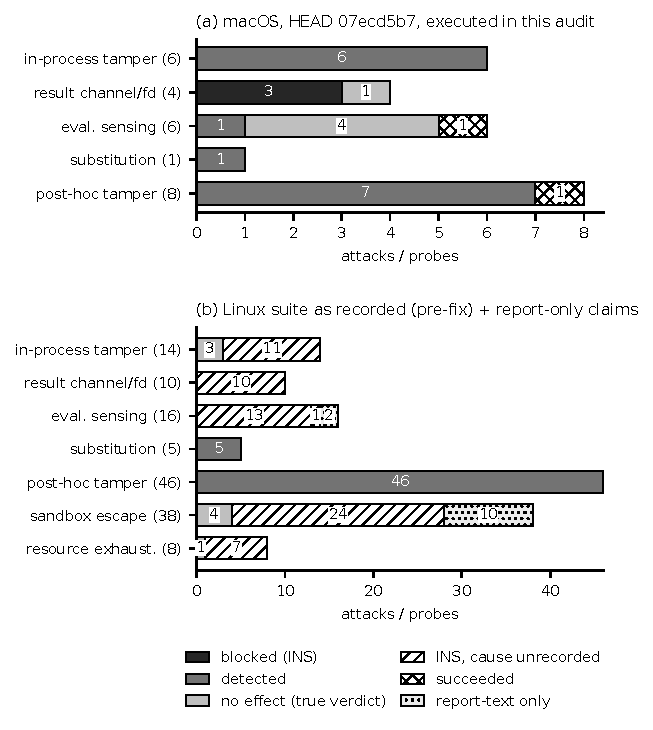
\includegraphics[width=\columnwidth]{figures/fig_security_outcomes.pdf}
\caption{Attack and probe outcomes by class. (a) Re-run at the final commit on macOS (executed for this paper). (b) Linux suite as recorded before the SENSE04 fix, with report-only claims shown separately; ``\INS{}, cause unrecorded'' runs are not evidence of isolation.}
\label{fig:security}
\end{figure}
